%\documentclass[t,10pt]{beamer}
\documentclass[t,handout]{beamer}

\usepackage{graphicx}
\usepackage{epsfig}
\usepackage{psfrag}
\usepackage[english]{babel}
\usepackage{color}
\usepackage{natbib}
\usepackage{booktabs}
\usepackage{listings}

% Font settings:
\usepackage[T1]{fontenc}
\usepackage{mathptmx}
\usepackage[scaled]{helvet}
\usepackage{courier}
\usepackage{microtype}



%Mathematics packages
\usepackage{amsmath}
\usepackage{mathrsfs}
\usepackage{amsfonts}
\usepackage{enumerate}

\graphicspath{{./images/}} % Figures path - used in graphicx

\selectcolormodel{cmyk}

\mode<presentation>

%THEMES - Please refer to these chapters in the beamer documentation.
% Presentation themes : Chapter 15
% Color themes : Chapter 17
% Font themes : Chapter 18
\usetheme{Pittsburgh}
\usecolortheme{orchid}
\usefonttheme{default}

\setbeamertemplate{bibliography item}[text]
\setbeamercovered{transparent=7}

%---------------------------Title frame definition------------------------------------- 

\title{Information Protection in Content-centric Networks}
\author [Chris]{Christopher C. Lamb}
\institute[University of New Mexico]{
\inst {}Department of Electrical and Computer Engineering\\
University of New Mexico}
\date{November 6, 2012}
\titlegraphic{
\begin{figure} 

\includegraphics[width = 7cm]{unm-logo}
\end{figure}}

% Delete this, if you do not want the table of contents to pop up at
% the beginning of each subsection:
%\AtBeginSubsection[]
%{
%  \begin{frame}<beamer>
%    \frametitle{Outline}
%     \tableofcontents[currentsection,currentsubsection]
%  \end{frame}
%}

\begin{document}

\begin{frame}
\titlepage
\end{frame}

% This command will make the logo appear on all frames excluding the title frame.
\logo {
\includegraphics[width = 2.5cm]{unm-logo}}

\begin{frame}[t]
\frametitle{Outline}
\tableofcontents 
\end{frame}

%\input{content-slides/summary}

\section{Summary}

\begin{frame}
\frametitle{Definitions}
There are a few different definintions of {\bf Assured Information Sharing}: \\
\begin{itemize}
\item {\small The DoD's vision for AIS is to {\sl "deliver the power of information to ensure mission success through an agile enterprise with freedom of maneuverability across the information environment"}}
\item {\small Daniel Wolfe (formerly of the NSA) defined assured information sharing (AIS) as a framework that {\sl "provides the ability to dynamically and securely share information at multiple classification levels among U.S., allied and coalition forces."}}
\item {\small For the scope of Nublu: {\sl A modern computer system capable of dynamically and securely managing delivery and use of open and sensitive information to U.S., Allied, and Coalition partners when and where the partners need it, in a form they can use, to provide an asymmetric operational advantage to U.S. affiliated forces.}}
\end{itemize}
\end{frame}

\begin{frame}
\frametitle{Definitions}
So what does this mean? \\
\begin{itemize}
\item {\small {\bf Modern computer system} --- cloud based; we'll use openstack as it is what MilCloud is based on and we want to integrate with this to have a chance for Phase III.}
\item {\small {\bf dynamically and securely managing delivery and use} --- providing the ability to {\sl autonomously} provide and retract access to information based on {\sl changing properties} of that information, the environment, and system users.  The information must be delivered respecting defined {\sl confidentiality}, {\sl integrity}, {\sl availability}, {\sl urgency}, and {\sl importance} requirements.}
\end{itemize}
\begin{beamerboxesrounded}[shadow]{CIA isn't sufficient}
{\small CIA is not enough; need some idea of information importance and urgency too.}
\end{beamerboxesrounded}
\end{frame}

\section{Phase I}

\begin{frame}
\frametitle{Phase I Goals}
{\bf Original Concept of Operations} --- resource access and virtual machine instantiation is a function of user authorization, operating context, resource attributes, and usage policies.  Phase II builds on phase I via:
\begin{itemize}
{\small
\item \textit{\textbf{Confidentiality}} --- Data object key management, user key management, homomorphic encryption
\item \textit{\textbf{Integrity}} --- Individual and Group signature schemes, integrated integrity verification checking
\item \textit{\textbf{Availability}} --- Hardened instances, redundant images
}
\end{itemize}
Other areas of work include robust, graduated logging and auditing.

\begin{beamerboxesrounded}[shadow]{Usage Management System}
{\small Controls the initial resource access and cloud computing system provisioning.
Monitors the resource security parameters, cloud computing resource security characteristics, and operator context to provide continuous control.}
\end{beamerboxesrounded}

\end{frame}

\begin{frame}
\frametitle{Operation --- Initial Configuration}
\begin{figure}[!t]
\centering
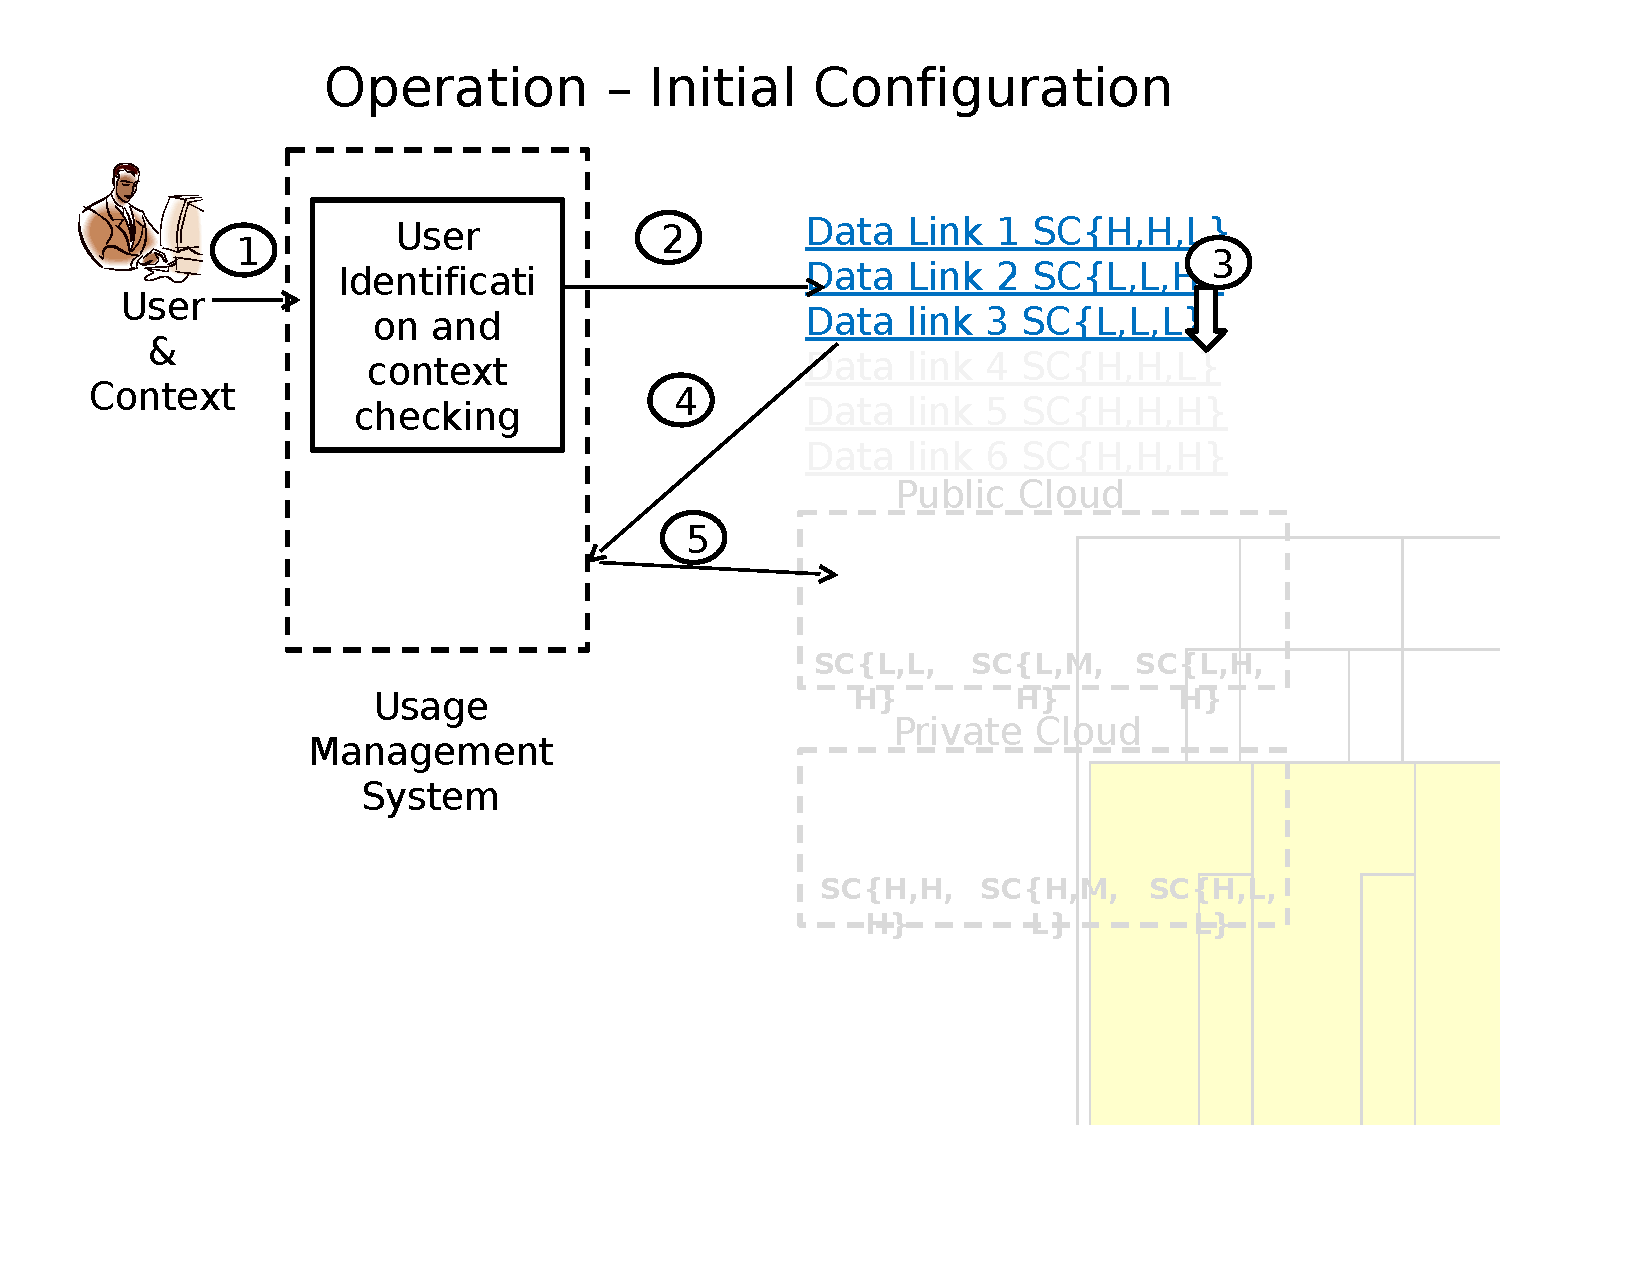
\includegraphics[width=\textwidth]{3}
\end{figure}
\end{frame}

\begin{frame}
\frametitle{Operation --- Dynamic Re-configuration 1}
\begin{figure}[!t]
\centering
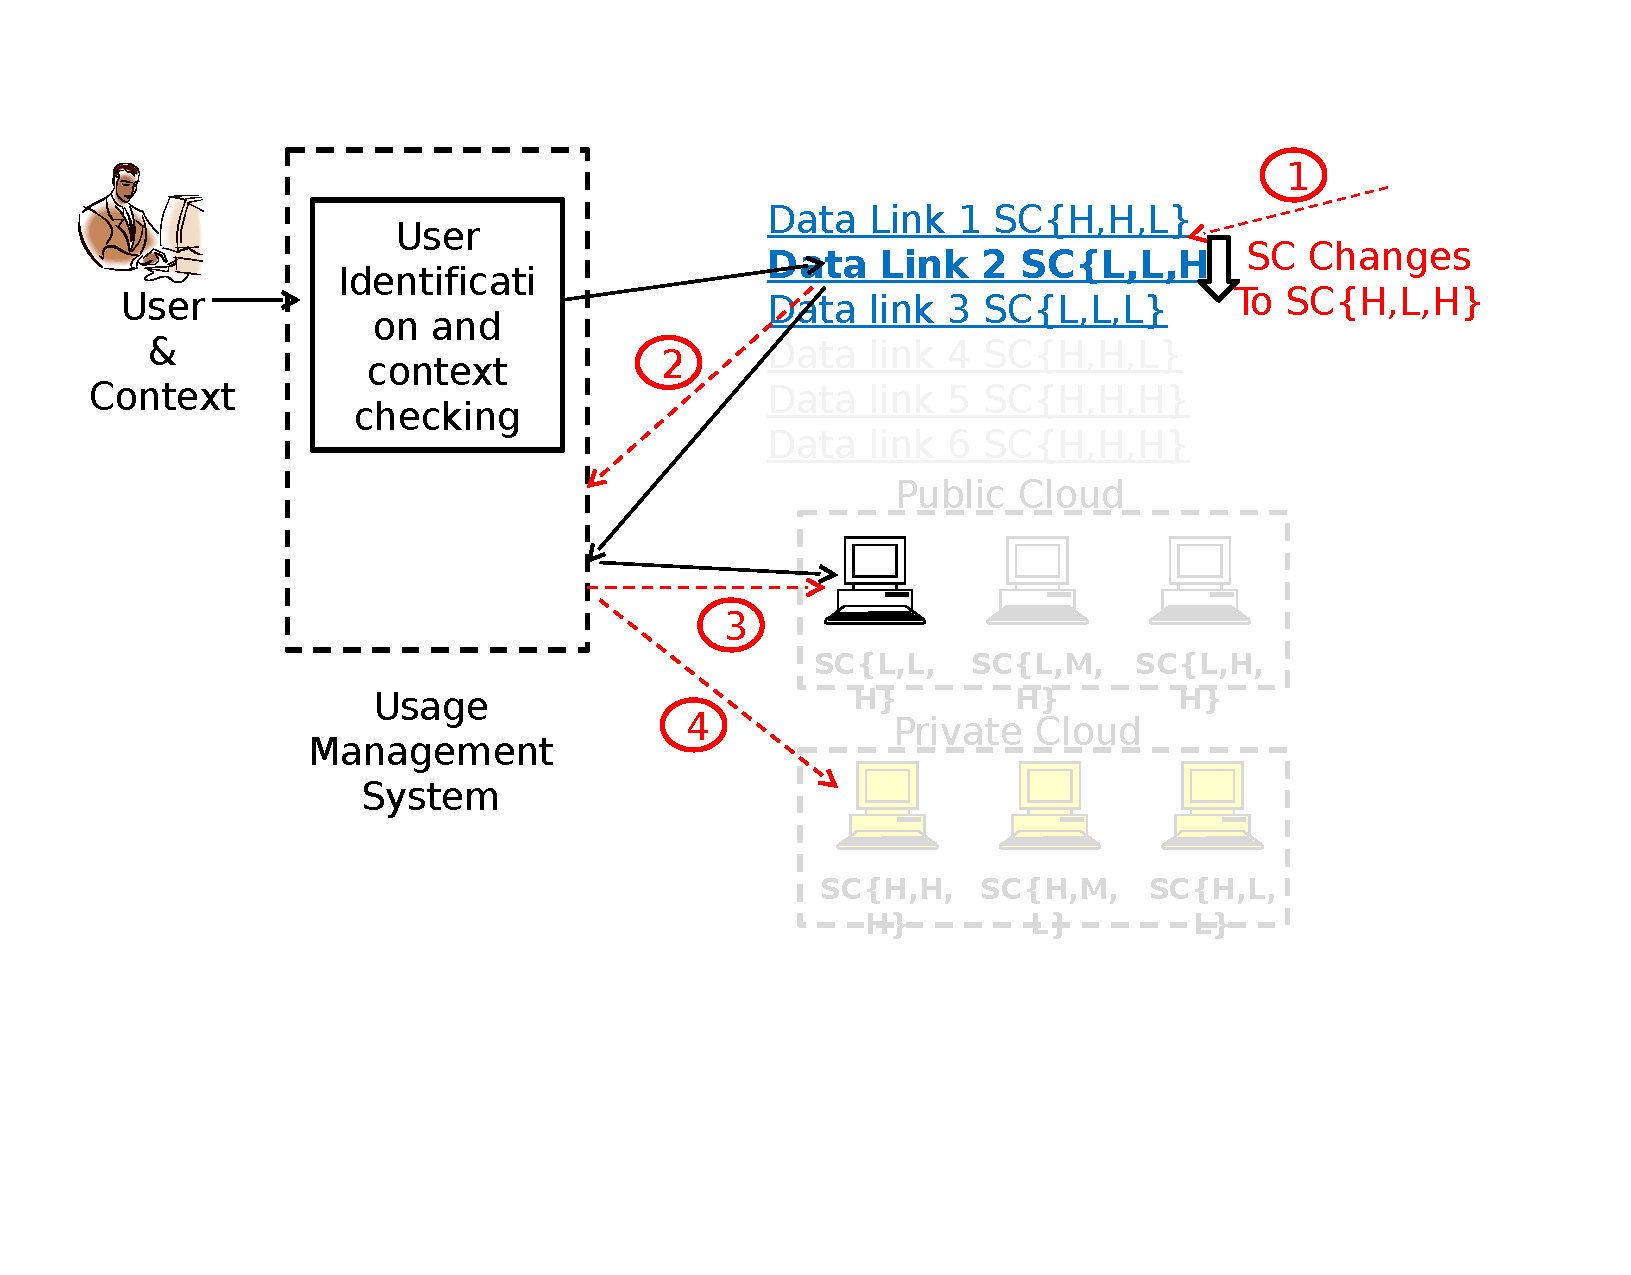
\includegraphics[width=\textwidth]{4}
\end{figure}
\end{frame}

\begin{frame}
\frametitle{Operation --- Dynamic Re-configuration 2}
\begin{figure}[!t]
\centering
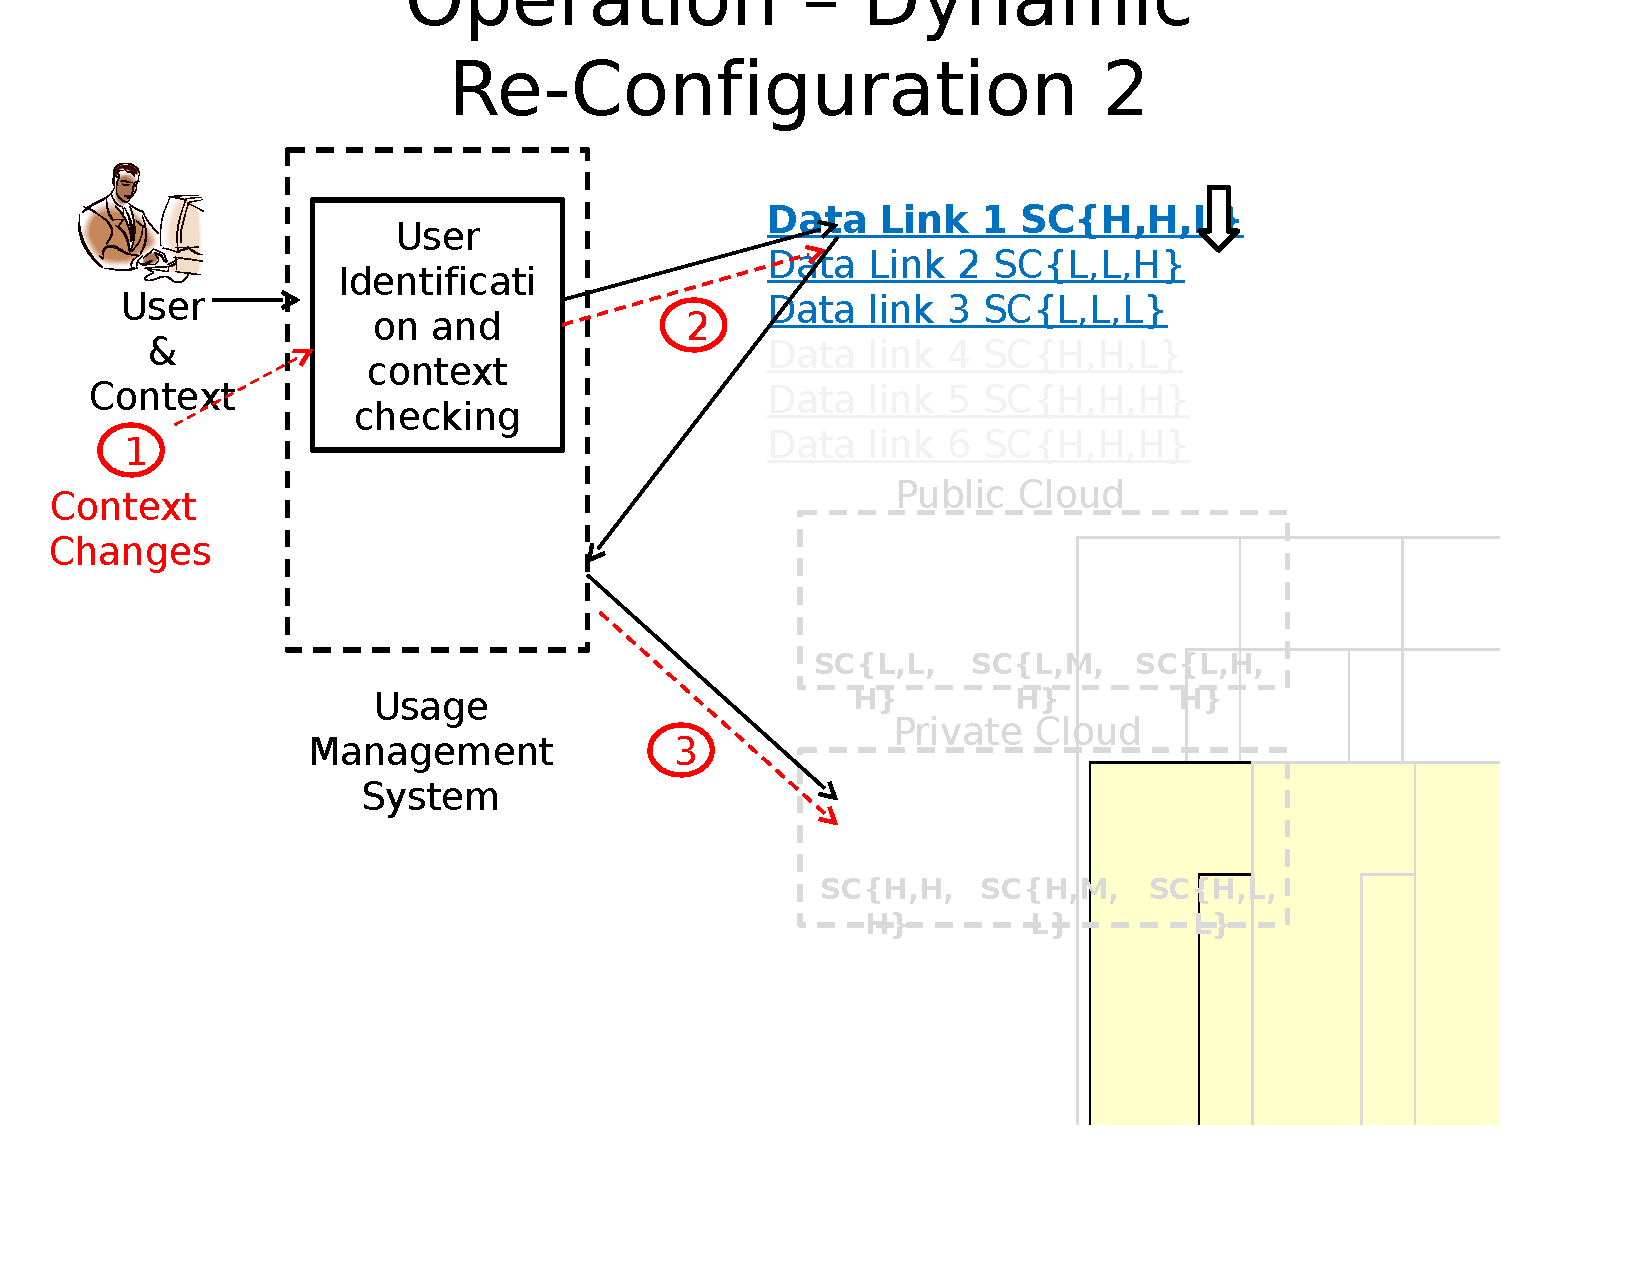
\includegraphics[width=\textwidth]{5}
\end{figure}
\end{frame}

\begin{frame}
\frametitle{Operation --- Usage Management}
\begin{figure}[!t]
\centering
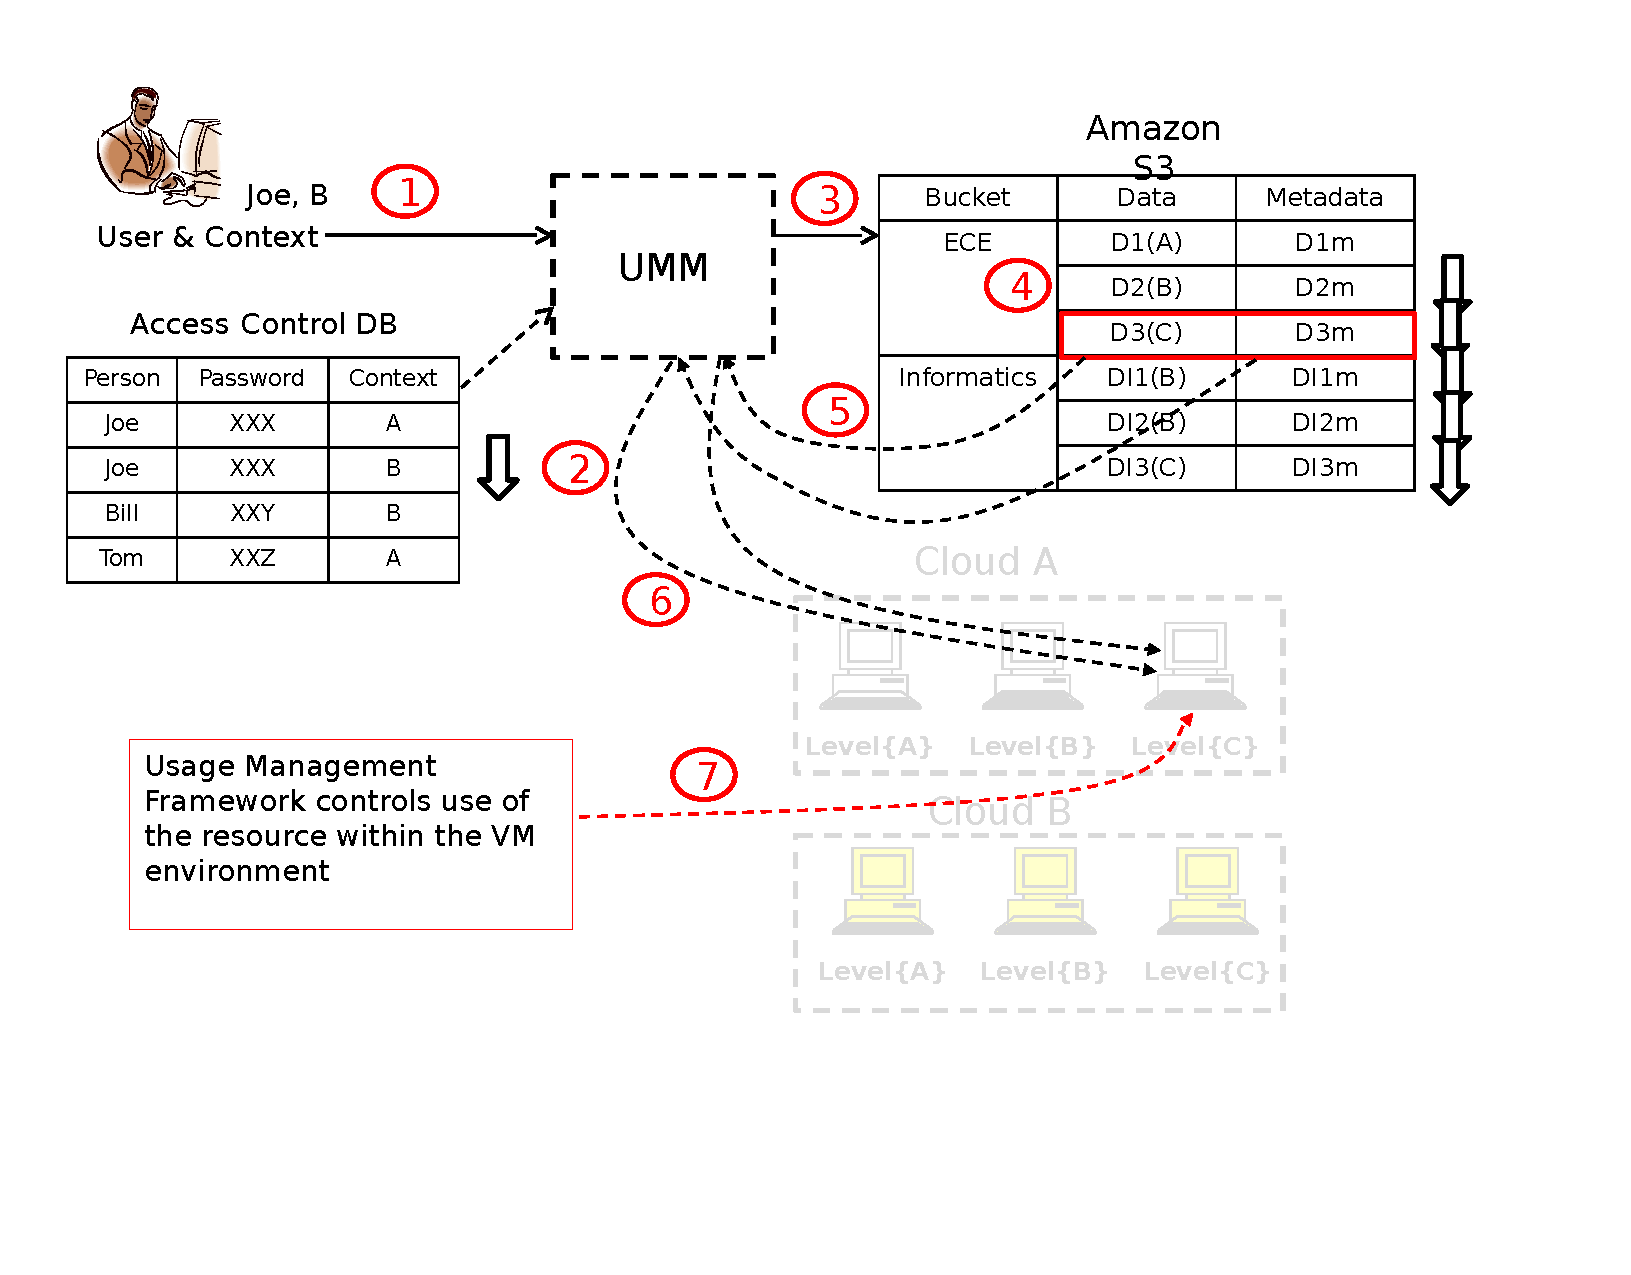
\includegraphics[width=\textwidth]{6}
\end{figure}
\end{frame}

\begin{frame}
\frametitle{Operation --- Dynamic Re-configuration 3}
\begin{figure}[!t]
\centering
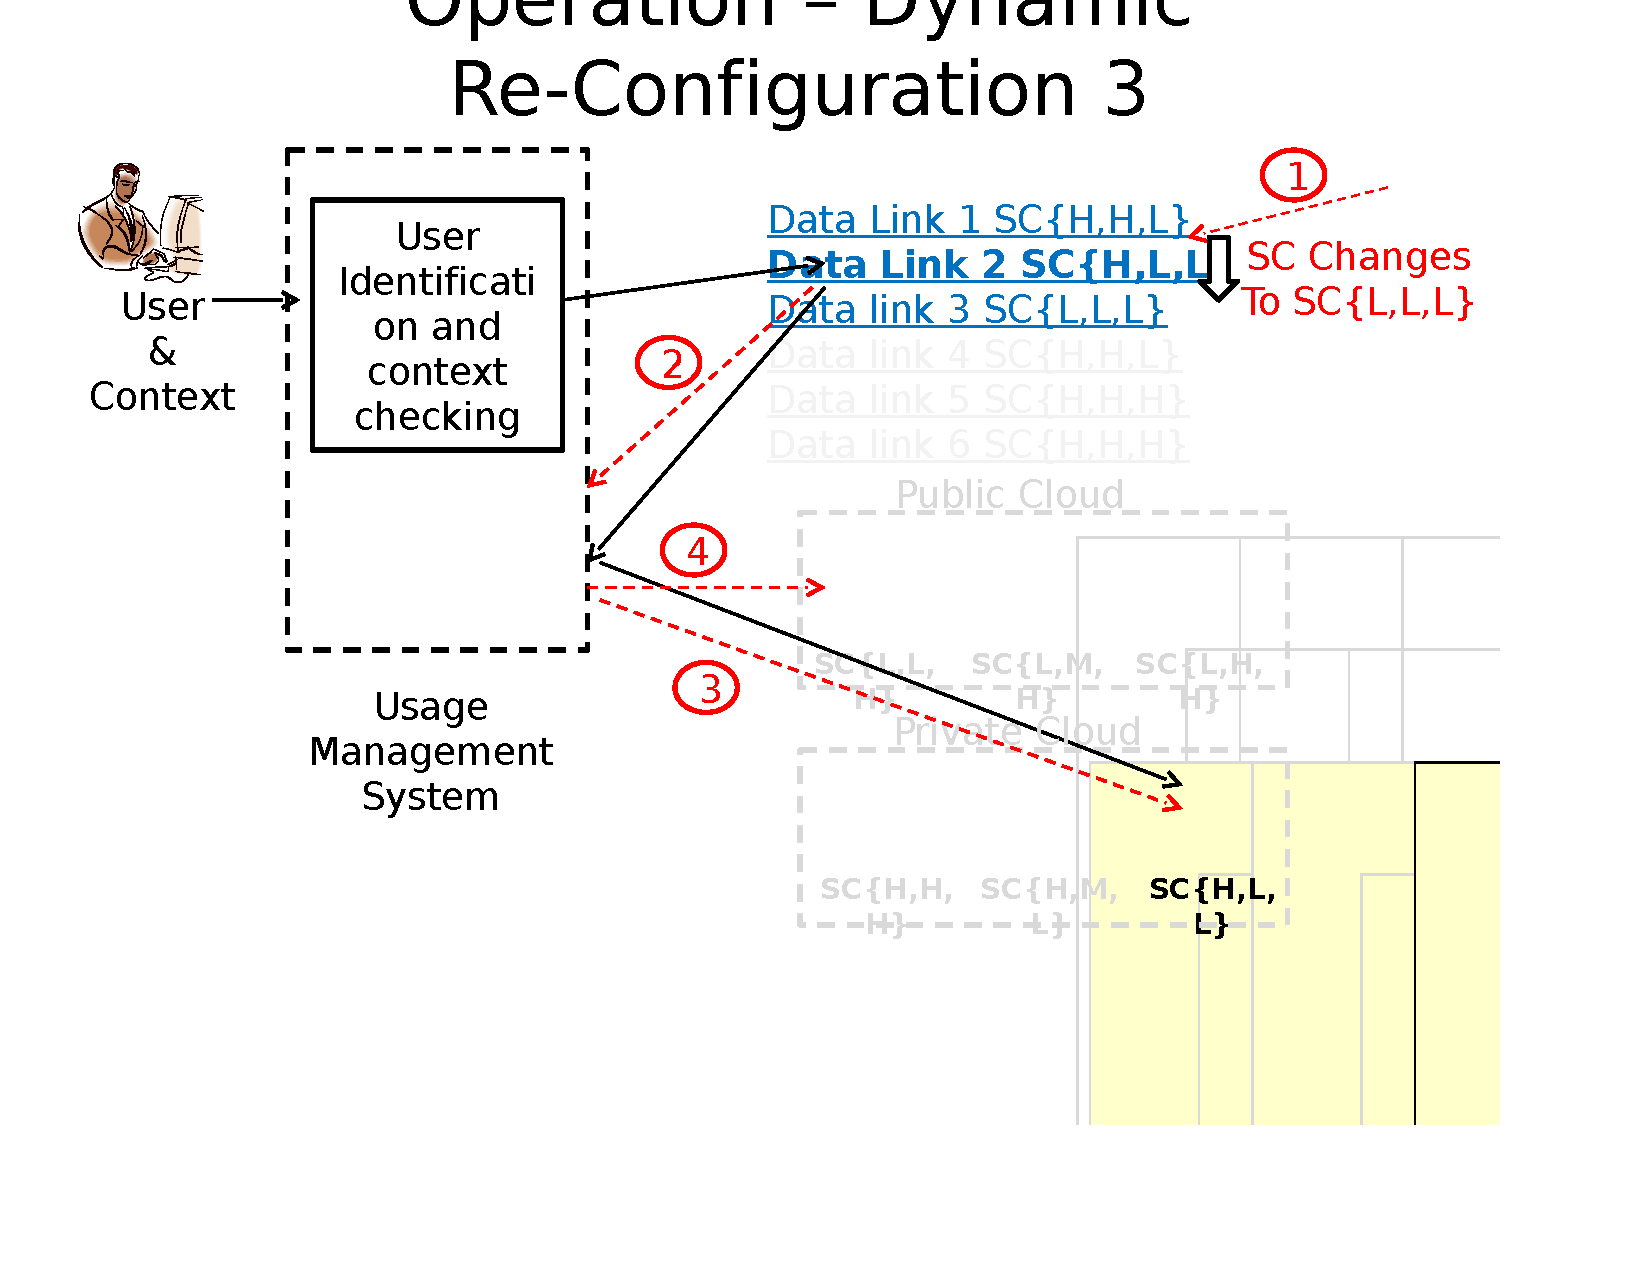
\includegraphics[width=\textwidth]{7}
\end{figure}
\end{frame}

\begin{frame}
\frametitle{Building on Phase I}

\end{frame}

\begin{frame}
\frametitle{Span of Control --- IaaS}
\begin{figure}[!t]
\centering
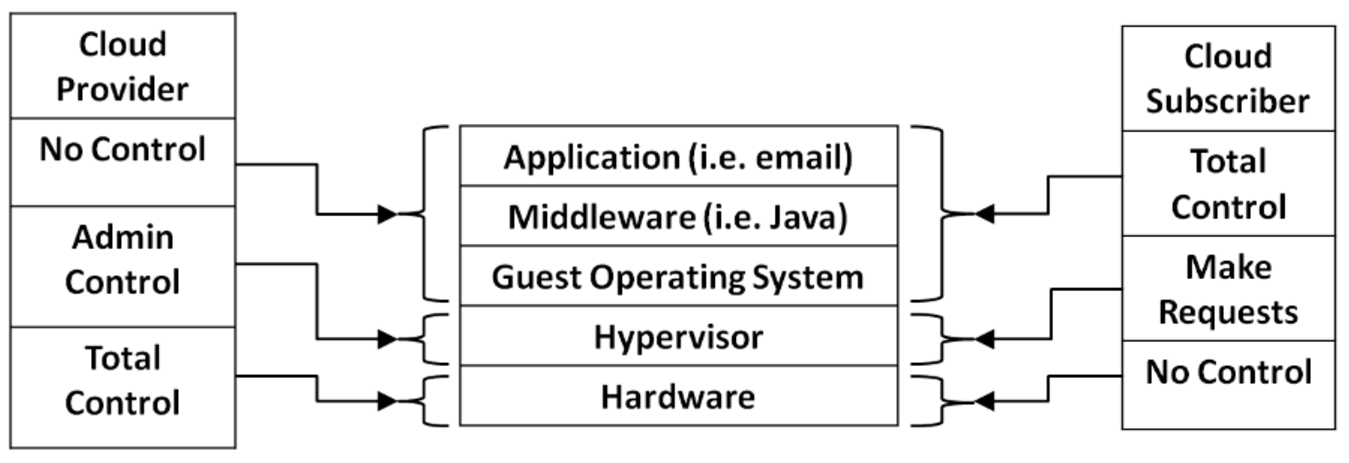
\includegraphics[width=\textwidth]{8-crop}
\end{figure}
\end{frame}

\begin{frame}
\frametitle{Application Software and OS}
\begin{figure}[!t]
\centering
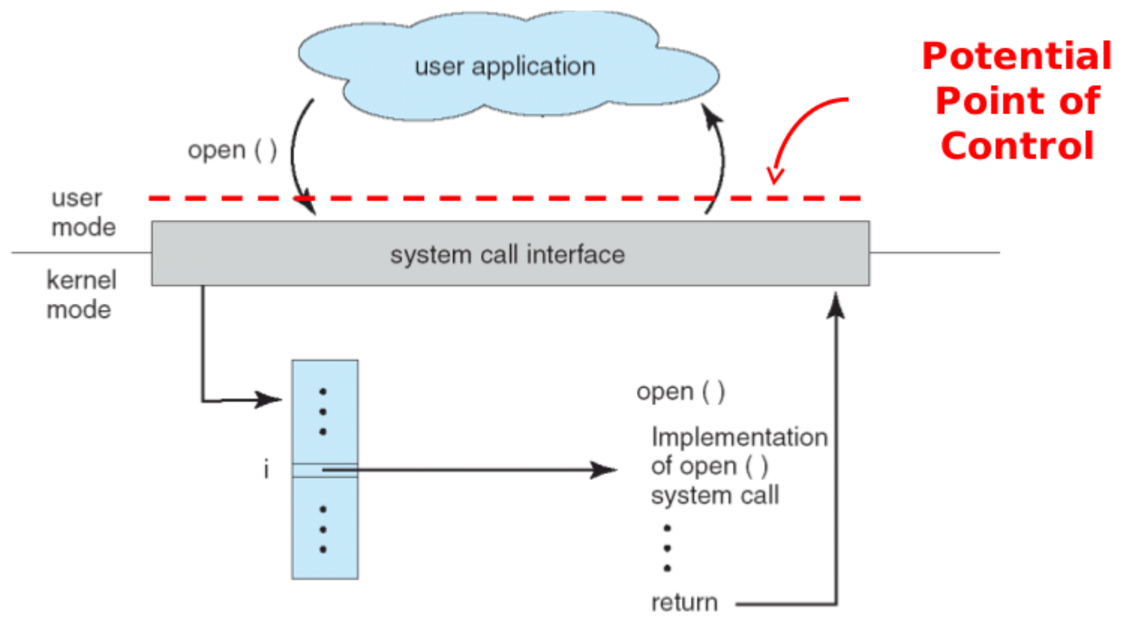
\includegraphics[width=\textwidth]{9-crop}
\end{figure}
\end{frame}

\begin{frame}
\frametitle{Layering with VMWare}
\begin{figure}[!t]
\centering
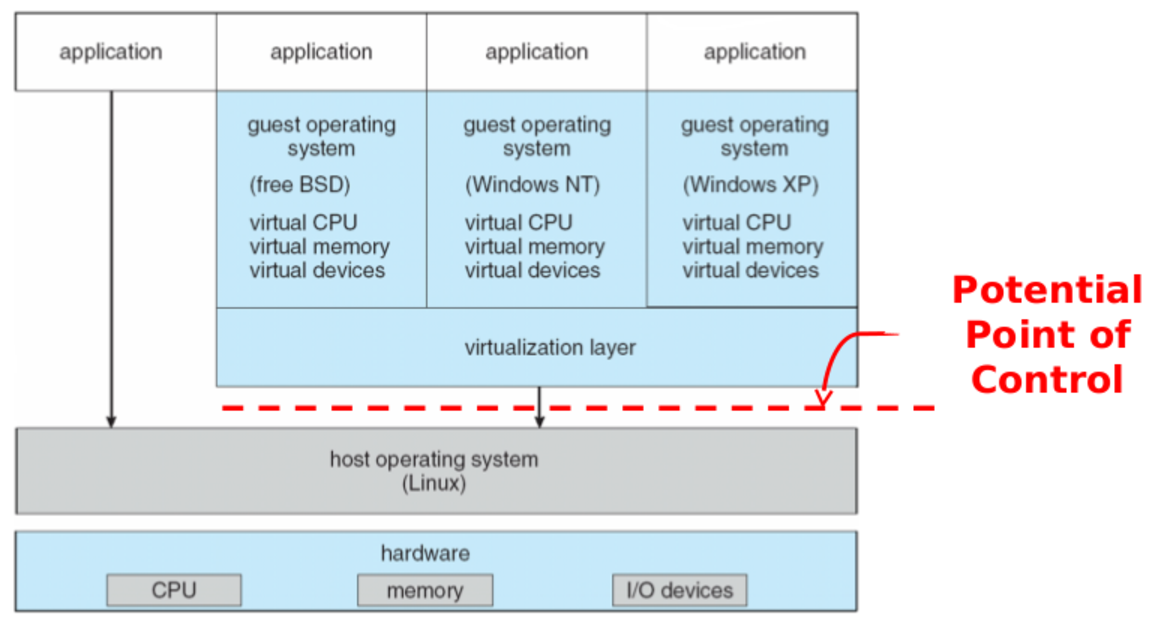
\includegraphics[width=\textwidth]{10-crop}
\end{figure}
\end{frame}

\begin{frame}
\frametitle{Key Considerations}
\begin{itemize}
\item The interfaces between the application and operating system, and between the operating system and the hardware, lend themselves to the introduction of control functions.
\item It is highly undesirable to modify the operating system itself because of the size and complexity.
\item It is also undesirable to modify application software.
\item Hardware components like the TPM can provide extremely useful capabilities in private cloud environments.
\item Encryption is a key element in information security.Partially homomorphic encryption can be useful in some applications, but is not a universal solution.
\item Isolation methods using nested virtualization are very useful.
\item Key management procedures and certificates will be essential.
\end{itemize}
\end{frame}

\begin{frame}
\frametitle{What else will we not do?}
We are to provide a cloud-based system integrable with MilCloud that supports these goals.  We will not:
\begin{itemize}
\item Provide last-mile data consumption
\item Develop sensor networks
\end{itemize}
\begin{beamerboxesrounded}[shadow]{Still...}
{\small We need to be able to take data from sensor networks and deliver information to mobile consumers. This implies some kind of {\sl very simple} mobile client emulated sensor input.}
\end{beamerboxesrounded}
\end{frame}

\section{Use Cases}

\begin{frame}
\frametitle{Attributes of Use Cases}
Use cases embody:
\begin{itemize}
\item {\bf Who} --- U.S., Allied, Coalition
\item {\bf What} --- managing sensitive and open information (giving, limiting, or denying access), impact of environmental attributes, bursting based on performance, differential security control application
\item {\bf When} --- time bounds on information delivery
\item {\bf Where} --- Geographic bounds on information dissemination
\item {\bf Why} --- N/A
\item {\bf How} --- Dynamically and Securely, other
\end{itemize}
\end{frame}

\section{System}

\begin{frame}
\frametitle{Building Blocks and Strategy}
{\bf Strategy}: Use functional partitioning to simplify overall architecture and issue traceability. Some examples:
\begin{itemize}
{\small 
\item {\bf Enclaves} --- Dedicated environments providing processing, networking, or storage services.
\item {\bf Processing} --- Processing nodes of various sizes and configurations, hosted in various enclaves.
\item {\bf Networking} --- Networks connecting nodes using overlays and differential routing supplying different protection schemes.
\item {\bf Storage} --- Storage using different approaches and security profiles.  Includes primary (repositories) and secondary (caches) storage.
\item {\bf Information} --- Meaningful data of different types (e.g. streaming, structured, document-based.
\item {\bf Policies} --- Policies describing use of information.
}
\end{itemize}
Attributes? Internal and external structures? Security Models?
\end{frame}

\begin{frame}
\frametitle{Information Objects}
Start with an {\sl Information Object}.\\~\\

This is a resource that contains valuable, managed data.\\~\\

Protected it via encryption, and digitally sign the encrypted information object. \\~\\

Now, the {\sl information object} has become a {\sl protected information object}.  This package can then be stored in any number of object or document-centric storage schemes common in cloud environments.\\~\\

Policies are associated with protected information objects, forming {\sl protected information packages}.  Policies are not encrypted.

{\sl Integrate open and closed source encryption algorithms.  Can we maintain secret inputs? }
\end{frame}

\begin{frame}
\frametitle{Virtual Networking}
The protected information package moves through securely provisioned {\sl virtual networks}.  These networks are configured with strong encryption, and involve only those parties that need access to the distributed information.  They are configured dynamically, when needed.  They are multiplexed over shared physical infrastructure.

{\sl SDN and pop-up VLANS?}
\end{frame}

\begin{frame}
\frametitle{Policy Enforcement}
Distribution and policy enforcement is handled by a {\sl usage management mechanism}.  This usage management mechanism acts as both a policy decision point and a policy enforcement point. \\~\\

This component can filter and modify content based on dynamic subject, environment, and resource centric policies. It furthermore is closely coupled to any PKI systems, and can extract, repackage, and re-sign any content en-route to a specified destination.\\~\\

We have policy enforcement throughout the system.\\~\\

{\sl Can we maintain secret inputs here too? How to manage keys and encryption algorithms?}
\end{frame}

\begin{frame}
\frametitle{Processing}
Processing nodes receive data and are able to commence processing.  These nodes are virtualized.  \\~\\

Nodes may either control computation via internal usage management, or be configured to handle information at a specific sensitivity level, or both. \\~\\

{\sl bursting?}
\end{frame}

\begin{frame}
\frametitle{Delivery and Consumption}
Thick clients, web, mobile
\end{frame}

\begin{frame}
\frametitle{SIEM}
Logly, others?
\end{frame}

\begin{frame}
\frametitle{Other Concerns}
system and data security models?
\end{frame}

\section{Use Case Traceability}

%\begin{frame}
%\frametitle{Possible Research Topics}
%\begin{itemize}
%\item In VM usage management, or dedicated VM instances?
%\item Cross Domain Communication Surfaces and Design
%\item Controllable Bursting System Design  (inter- and intra- cloud)
%\item Provisionable, dynamic network security
%\item Data Management Standards: Rest, Motion, Use
%\item Cloud Confidentiality, Integrity, Availability Strategies and Costs
%\item SEIM Cloud Solutions and Architectures: How to build?
%\item Implications of the Last Mile: Delivering Sensitive Info to Mobile Devices
%\item System and Data Security Models and Implications
%\end{itemize}
%\end{frame}



\end{document}